\documentclass{article}
% \usepackage[headsepline]{scrlayer-scrpage}

% \ihead{Levin}
% \ohead{\thepage}
% \pagestyle{scrheadings}
\usepackage{bbm}
\usepackage{amsmath,amsfonts,amsthm,amssymb,amsopn,bm}
\usepackage[margin=.9in]{geometry}
\usepackage{graphicx}
\usepackage{url}
\usepackage[usenames,dvipsnames]{color}
\usepackage{fancyhdr}
\usepackage{multirow}

\usepackage{pgfplots}

% Some additional tweaking for this package can be made in the preamble. To change the size of each plot and also guarantee backwards compatibility (recommended) add the next line:

\pgfplotsset{width=10cm,compat=1.9}

% This changes the size of each pgfplot figure to 10 centimeters, which is huge; you may use different units (pt, mm, in). The compat parameter is for the code to work on the package version 1.9 or later.

% Since LaTeX was not initially conceived with plotting capabilities in mind, when there are several pgfplot figures in your document or they are very complex, it takes a considerable amount of time to render them. To improve the compiling time you can configure the package to export the figures to separate PDF files and then import them into the document, add the code shown below to the preamble:

\usepgfplotslibrary{external}

\tikzexternalize 

\newcommand{\field}[1]{\mathbb{#1}}
\newcommand{\1}{\mathbf{1}}
\newcommand{\I}{\mathbbm{1}}
\newcommand{\E}{\mathbb{E}} 
\newcommand{\V}{\mathbb{V}} 
\renewcommand{\P}{\mathbb{P}}
 \newcommand{\ind}{\perp\!\!\!\perp}
 \DeclareMathOperator{\rank}{rank}
\newcommand{\R}{\field{R}} % real domain
% \newcommand{\C}{\field{C}} % complex domain
\newcommand{\F}{\field{F}} % functional domain

\newcommand{\T}{^{\textrm T}} % transpose

\def\diag{\text{diag}}

%% operator in linear algebra, functional analysis
\newcommand{\inner}[2]{#1\cdot #2}
\newcommand{\norm}[1]{\left\|#1\right\|}
\newcommand{\twonorm}[1]{\|#1\|_2^2}
% operator in functios, maps such as M: domain1 --> domain 2
\newcommand{\Map}[1]{\mathcal{#1}}
\renewcommand{\theenumi}{\alph{enumi}} 

\newcommand{\Perp}{\perp \! \! \! \perp}

\newcommand\independent{\protect\mathpalette{\protect\independenT}{\perp}}
\def\independenT#1#2{\mathrel{\rlap{$#1#2$}\mkern2mu{#1#2}}}
\newcommand{\vct}[1]{\boldsymbol{#1}} % vector
\newcommand{\mat}[1]{\boldsymbol{#1}} % matrix
\newcommand{\cst}[1]{\mathsf{#1}} % constant
\newcommand{\ProbOpr}[1]{\mathbb{#1}}
\newcommand{\points}[1]{\small\textcolor{magenta}{\emph{[#1 points]}} \normalsize}
\date{{}}

\setlength\parindent{0px}

\begin{document}
\title{Homework \#0}
\author{\normalsize{Spring 2020, CSE 546: Machine Learning}\\
\normalsize{\bf Roman Levin} \\
\normalsize{\bf 1721898} \\
}
\maketitle

\section*{Problems A}
\subsection*{Probability and Statistics}
A.1 \points{2} (Bayes Rule, from Murphy exercise 2.4.) After your yearly checkup, the doctor has bad news and good news. The bad news is that you tested positive for a serious disease, and that the test is 99\% accurate (i.e., the probability of testing positive given that you have the disease is 0.99, as is the probability of testing negative given that you dont have the disease). The good news is that this is a rare disease, striking only one in 10,000 people. What are the chances that you actually have the disease? (Show your calculations as well as giving the final result.)\\
\\
\noindent\rule{\textwidth}{1pt}
{\bf Solution:}\\
\\
Denote "+" the event of a positive test, denote "-" the event of a negative test, denote "disease" the event of having the disease, and denote "no disease" the event of not having the disease. Then, note that:
\begin{itemize}
    \item $\mathbb{P}(+\vert \text{disease}) = 0.99$
    \item $\mathbb{P}(-\vert \text{no disease}) = 0.99 \Rightarrow \mathbb{P}(+\vert \text{no disease}) = 1 - \mathbb{P}(-\vert \text{no disease}) = 0.01$
    \item $\mathbb{P}(\text{disease}) = 10^{-4} \Rightarrow \mathbb{P}(\text{no disease}) = 1 - \mathbb{P}(\text{disease}) = 0.9999$ 
\end{itemize}
By the total probability law, we can find:
\begin{equation}\label{+}
    \mathbb{P}(+) = \mathbb{P}(+\vert \text{disease})\mathbb{P}(\text{disease}) +  \mathbb{P}(+\vert \text{no disease})\mathbb{P}(\text{disease})  
\end{equation}
Then, using the equation \eqref{+} and Bayes rule, we obtain:
\begin{equation}\boxed{
\begin{split}
    &\mathbb{P}(\text{disease} \vert +) = \frac{\mathbb{P}(+\vert \text{disease})\mathbb{P}( \text{disease})}{\mathbb{P}(+)} = \frac{\mathbb{P}(+\vert \text{disease})\mathbb{P}( \text{disease})}{\mathbb{P}(+\vert \text{disease})\mathbb{P}(\text{disease}) +  \mathbb{P}(+\vert \text{no disease})\mathbb{P}(\text{disease})} =\\
    &= \frac{0.99\cdot0.0001}{0.99\cdot0.0001 + 0.01\cdot0.9999} = \frac{1}{102}
\end{split}}
\end{equation}

\noindent\rule{\textwidth}{1pt}


A.2 For any two random variables $X,Y$ the \emph{covariance} is
  defined as
  $\text{Cov}(X,Y)=\E[(X-\E[X])(Y-\E[Y])]$. You may assume $X$ and $Y$
  take on a discrete values if you find that is easier to work with.
\begin{enumerate}
\item \points{1} If $\E[Y|X=x] = x$ show that $\text{Cov}(X,Y) = \E[(X-\E[X])^2]$.  
\\
\\
\noindent\rule{\textwidth}{1pt}
{\bf Solution:}\\
\\
Probably, a better way to solve this would be to use iterated expectation and conditioning on $X$ as an RV (not on the event $X=x$), but I am not sure if $\E[Y|X] = X$ follows from the problem statement, so I will just assume $X$ and $Y$ are discrete RVs. Then:
\begin{itemize}
    \item By linearity of expectation: $\text{Cov}(X,Y)=\E[(X-\E[X])(Y-\E[Y])] = \E[XY] - \E[X\E[Y]] - \E[\E[X]Y] + \E[X]\E[Y] = \E[XY] - \E[X]\E[Y]$ 
    
    \item By the law of total expectation: $\E[XY] = \sum_x \mathbb{P}(X=x)\E[XY\vert X=x] = $\\$ =\sum_x \mathbb{P}(X=x)x\E[Y\vert X=x] = \sum_x \mathbb{P}(X=x)x^2 = \E[X^2]$
    \item By the law of total expectation: $\E[Y] = \sum_x \mathbb{P}(X=x)\E[Y\vert X=x] = \sum_x \mathbb{P}(X=x)x = \E[X]$
\end{itemize}
Combining the above, we get:
$$\text{Cov}(X,Y) = \E[X^2] - (\E[X])^2 = \E[(X-\E[X])^2] \qquad \Box$$



\noindent\rule{\textwidth}{1pt}

\item \points{1} If $X,Y$ are independent show that $\text{Cov}(X,Y)=0$.
\\
\\
\noindent\rule{\textwidth}{1pt}
{\bf Solution:}\\
\begin{itemize}
    \item In a. we have shown: $\text{Cov}(X,Y)= \E[XY] - \E[X]\E[Y]$ 
    \item Since $X$ and $Y$ are independent: $\E[XY] = \sum_{x,y}\mathbb{P}(X=x, Y= y)xy = \sum_{x,y}\mathbb{P}(X=x)\mathbb{P}(Y= y)xy = \left(\sum_{y}\mathbb{P}(X=x)x\right)\left(\sum_{y}\mathbb{P}(Y= y)y\right) = \E[X]\E[Y]$
\end{itemize}
Combining the above, we get $$\text{Cov}(X,Y) = 0 \qquad \Box$$

\noindent\rule{\textwidth}{1pt}

\end{enumerate}


A.3 Let $X$ and $Y$ be independent random variables with PDFs given by $f$ and $g$, respectively. Let $h$ be the PDF of the random variable $Z = X+Y$.
\begin{enumerate}
	\item \points{2} Show that $h(z) = \int_{-\infty}^\infty f(x) g( z - x ) d x $.  (If you are more comfortable with discrete probabilities, you can instead derive an analogous expression for the discrete case,  and then you should give a one sentence explanation as to why your expression is analogous to the continuous case.).
	\\
    \\
    \noindent\rule{\textwidth}{1pt}
    {\bf Solution:}\\
    \begin{itemize}
        \item Joint PDF of $X,Y$: $X \ind Y \Rightarrow f_{X,Y}(x,y) = f(x)g(y)$
        \item $F_Z(z) = \P(Z\le z) = \P(X+Y \le z) = \iint_{x+y \le z} f_{X,Y}(x,y)dx dy = \int_{-\infty}^{\infty}\left(\int_{-\infty}^{z-x} f(x)g(y)dy\right)dx = \int_{-\infty}^{\infty}f(x)\left(\int_{-\infty}^{z-x} g(y)dy\right)dx =  \int_{-\infty}^{\infty}f(x)F_Y(z-x)dx$
        \item $h(z) = \frac{d}{dz} F_Z(z) = \frac{d}{dz}\int_{-\infty}^{\infty}f(x)F_Y(z-x)dx = \int_{-\infty}^{\infty}f(x)\frac{d}{dz}F_Y(z-x)dx = \int_{-\infty}^{\infty}f(x)g(z-x)dx \qquad \Box$
    \end{itemize}


    \noindent\rule{\textwidth}{1pt}
	
	\item \points{1} If $X$ and $Y$ are both independent and uniformly distributed on $[0,1]$ (i.e. $f(x)=g(x)=1$ for $x \in [0,1]$ and $0$ otherwise) what is $h$, the PDF of $Z=X+Y$?
	\\
    \\
    \noindent\rule{\textwidth}{1pt}
    {\bf Solution:}\\
    Notation: $\I_{\{\cdot\}}$ stands for an indicator function.
    \begin{itemize}
        \item $g(x) = f(x) = \I_{ \{x \in [0,1] \} }$
        \item Plugging in to the result from a.: 
        \begin{equation}
        \begin{split}
        h(z)  & = \int_{-\infty}^{\infty}\I_{ \{x \in [0,1] \}}\I_{ \{z-x \in [0,1] \}}dx = \int_{-\infty}^{\infty}\I_{ \{x \in [0,1] \}}(\I_{ \{x \in (-\infty,z] \}}+\I_{ \{x \in [z-1,\infty) \}})dx =\\
        & = \int_0^1\I_{ \{x \in (-\infty,z] \}}dx + \int_0^1 \I_{ \{x \in [z-1,\infty) \}}dx = z\I_{ \{z \in [0,1] \}} + (2-z)\I_{ \{z-1 \in (0,1] \}}
        \end{split}
        \end{equation}
    \item This gives finally:
    $$
    \boxed{
    h(z) = 
    \begin{cases}
    z, &z \in [0,1] \\
    2-z, &z \in (1,2] \\
    0, &\text{o.w.}
    \end{cases}
    }
    $$
    \end{itemize}
    \noindent\rule{\textwidth}{1pt}
\end{enumerate}

A.4 \points{1} A random variable $X \sim \mathcal{N}(\mu, \sigma^2)$ is Gaussian distributed with mean $\mu$ and variance $\sigma^2$. Given that for any $a,b \in \R$, we have that $Y = aX + b$ is also Gaussian, find $a,b$ such that $Y \sim \mathcal{N}(0,1)$.\\
\\
\\
    \noindent\rule{\textwidth}{1pt}
    {\bf Solution:}\\
    Consider $$\boxed{a = \frac{1}{\sigma}, b = \frac{-\mu}{\sigma}}$$ 
    Then, since multiplying an RV by a constant multiplies the mean by the constant and the variance by the squared constant and since adding a constant to an RV shifts the mean by that constant and does not affect the variance:
    $$
    aX \sim \mathcal{N}(\frac{\mu}{\sigma}, 1) \text{  and  } Y \sim \mathcal{N}(0,1) \qquad \Box
    $$
    \noindent\rule{\textwidth}{1pt}
A.5 \points{2} For a random variable $Z$, its mean and variance are defined as $\E[Z]$ and $\E[(Z-\E[Z])^2]$, respectively.
Let $X_1,\dots,X_n$ be independent and identically distributed random variables, each with mean $\mu$ and variance $\sigma^2$. 
If we define $\widehat{\mu}_n = \frac{1}{n} \sum_{i=1}^n X_i$, what is the mean and variance of $\sqrt{n}(\widehat{\mu}_n - \mu)$?\\
\\
\\
    \noindent\rule{\textwidth}{1pt}
    {\bf Solution:}\\
    \begin{itemize}
    \item $\E[\sum_{i=1}^n X_i] = \sum_{i=1}^n \mu = \mu n$ and $\V[\sum_{i=1}^n X_i] = \sum_{i=1}^n \sigma^2 = \sigma^2 n$ since $X_i$ are iid.
    
    \item So $\E[\widehat{\mu}_n] = \mu$ and $\V[\widehat{\mu}_n] = \sigma^2/n$ (by the same argument with A.5).
    \item Then, again by the same argument with A.5: $$\boxed{\E(\sqrt{n}(\widehat{\mu}_n - \mu)) = 0, \V(\sqrt{n}(\widehat{\mu}_n - \mu)) = (\sqrt{n})^2\sigma^2/n = \sigma^2}$$
    \end{itemize}
    \noindent\rule{\textwidth}{1pt}
A.6 If $f(x)$ is a PDF, the cumulative distribution function (CDF)
  is  defined as $F(x) = \int_{-\infty}^x f(y) dy$.  For any function
  $g : \R \rightarrow \R$ and random variable $X$ with PDF $f(x)$,
  recall that the expected value of $g(X)$ is defined as
  $\E[g(X)] = \int_{-\infty}^\infty g(y) f(y) dy$. For a boolean event
  $A$, define $\1\{ A \}$ as $1$ if $A$ is true, and $0$
  otherwise. Thus, $\1\{ x \leq a \}$ is $1$ whenever $x \leq a$ and
  $0$ whenever $x > a$.  Note that $F(x) = \E[\1\{X \leq x\}]$.  Let
  $X_1,\dots,X_n$ be \emph{independent and identically distributed}
  random variables with CDF $F(x)$.  Define
  $\widehat{F}_n(x) = \frac{1}{n} \sum_{i=1}^n \1\{X_i \leq
  x\}$. Note, for every $x$,
  that $\widehat{F}_n(x)$ is an \emph{empirical estimate} of  $F(x)$.
  You may use your answers to the previous problem.
  \begin{enumerate}
  \item \points{1} For any $x$, what is $\E[ \widehat{F}_n(x) ]$?
  \\
\\
    \noindent\rule{\textwidth}{1pt}
    {\bf Solution:}\\
    $$\boxed{\E[ \widehat{F}_n(x) ] = \E [\frac{1}{n} \sum_{i=1}^n \1\{X_i \leq
  x\}] = \frac{1}{n} \sum_{i=1}^n \E [\1\{X_i \leq
  x\}] = \frac{1}{n} \sum_{i=1}^n F(x) = F(x)}$$
    
    \noindent\rule{\textwidth}{1pt}
  \item \points{1} For any $x$, the variance of $\widehat{F}_n(x)$ is $\E[ ( \widehat{F}_n(x) -
    F(x) )^2 ]$.  Show that $\textrm{Variance}(\widehat{F}_n(x)) = \frac{F(x)(1-F(x))}{n}$.
      \\
\\
    \noindent\rule{\textwidth}{1pt}
    {\bf Solution:}\\
    Since $X_i$ are iid, then $\1\{X_i < x\}$ are also independent as functions of $X_i$, thus we can write (also observing that $(\1\{X_i \leq x\})^2 = \1\{X_i \leq x\}$):
    \begin{equation}
    \begin{split}    
    \V[\widehat{F}_n(x)] &= \V [\frac{1}{n} \sum_{i=1}^n \1\{X_i \leq x\}] = 
    \frac{1}{n^2} \sum_{i=1}^n \V[\1\{X_i \leq x\}] =
    \frac{1}{n^2} \sum_{i=1}^n \left(\E[(\1\{X_i \leq x\})^2] - \E[\1\{X_i \leq x\}]^2\right) = \\
    & = \frac{1}{n^2} \sum_{i=1}^n \left(\E[\1\{X_i \leq x\}] - \E[\1\{X_i \leq x\}]^2\right) = \frac{1}{n^2} \sum_{i=1}^n \left(F(x) - F(x)^2\right) = \frac{F(x)(1-F(x))}{n} \qquad \Box
    \end{split}
    \end{equation}
    
    
    \noindent\rule{\textwidth}{1pt}
%    (Hint: Consider what independence implies.)
  \item \points{1} Using your answer to b, show that
    for all $x\in \R$, we have  $\displaystyle \E[ ( \widehat{F}_n(x) - F(x) )^2 ] \leq \tfrac{1}{4n}$.  
      \\
\\
    \noindent\rule{\textwidth}{1pt}
    {\bf Solution:}\\
    \begin{itemize}
        \item Note that $\E[\widehat{F}_n(x) - F(x)] = 0$ (from a.).
        \item Therefore  $\V[\widehat{F}_n(x) - F(x)] = \E[(\widehat{F}_n(x) - F(x))^2] = \frac{F(x)(1-F(x))}{n}$ (by b.)
        \item Since $F(x) \in [0,1] \forall x$, $\frac{F(x)(1-F(x))}{n}$ is maximized at $F(x) = \frac{1}{2}$ (it is just a parabola).
        \item Therefore $$\boxed{\E[(\widehat{F}_n(x) - F(x))^2] = \frac{F(x)(1-F(x))}{n} \leq \frac{0.5(1-0.5)}{n} = \frac{1}{4n} \qquad \Box}
        $$
    \end{itemize}    
    
    \noindent\rule{\textwidth}{1pt}
  \end{enumerate} 

B.1  \points{1} Let $X_1,\dots,X_n$ be $n$ independent and identically distributed random variables drawn unfiromly at random from $[0,1]$. If $Y = \max\{X_1,\dots,X_n\}$ then find $\E[Y]$.\\
\\
    \noindent\rule{\textwidth}{1pt}
    {\bf Solution:}\\
    Let $$F_X(x) = 
    \begin{cases}
    1, & x>1\\
    x, & x\in[0,1]\\
    0, & x<0
    \end{cases}
    $$ be the common CDF of $X_i$.
    \begin{itemize}
        \item Since $X_i$ are iid: $F_Y(y) = \P(Y \leq y) = \prod_{i=1}^n\P(X_i \le y) = \prod_i F_X(y) = F_X(y)^n$
        \item The PDF of Y:$f_Y(y) = \frac{d}{dy}F_Y(y) = \begin{cases}
    ny^{n-1}, & y\in[0,1]\\
    0, & \text{o.w}
    \end{cases}  $
    \item $$\boxed{\E[Y] = \int_0^1 yny^{n-1}dy = n\int_0^1 y^{n}dy = \frac{n}{n+1} }$$
    \end{itemize}
    \noindent\rule{\textwidth}{1pt}

\subsection*{Linear Algebra and Vector Calculus}
A.7 (Rank) Let $A = \begin{bmatrix} 1 & 2 & 1 \\ 1 & 0 & 3 \\ 1 & 1 & 2 \end{bmatrix}$ and $B = \begin{bmatrix} 1 & 2 & 3 \\ 1 & 0 & 1 \\ 1 & 1 & 2 \end{bmatrix}$.
For each matrix $A$ and $B$,
\begin{enumerate} 
	\item \points{2} what is its rank?\\
\\
    \noindent\rule{\textwidth}{1pt}
    {\bf Solution:}\\
    Let $a_i$ be the columns of A and $b_i$ be the columns of $B$.\\
    For A, observe that $-3a_1 + a_2 + a_3 = 0$ but any two columns are obviously linearly independent, so 
    $$
    \boxed{\rank{A} = 2}
    $$
    For B, observe that $b_3 - b_2 = b_1$ but any two columns are obviously linearly independent, so 
    $$
    \boxed{\rank{B} = 2}
    $$
    \noindent\rule{\textwidth}{1pt}
	\item \points{2} what is a (minimal size) basis for its column span?\\
\\
    \noindent\rule{\textwidth}{1pt}
    {\bf Solution:}\\
    For $A$, since its rank is 2 and $a_1, a_2$ are linearly independent, we can take $\{a_1, a_2\}$ as the basis for its column space.\\
    For $B$, since its rank is 2 and $b_1, b_2$ are linearly independent, we can take $\{b_1, b_2\}$ as the basis for its column space.
    
    \noindent\rule{\textwidth}{1pt}
\end{enumerate}

A.8 (Linear equations) Let $A = \begin{bmatrix} 0 & 2 & 4 \\ 2 & 4 & 2 \\ 3 & 3 & 1 \end{bmatrix}$, $b = \begin{bmatrix} -2 & -2 & -4 \end{bmatrix}^T$, and $c=\begin{bmatrix} 1 & 1 & 1 \end{bmatrix}^T$.
\begin{enumerate}
	\item \points{1} What is $Ac$?
	\\
\\
    \noindent\rule{\textwidth}{1pt}
    {\bf Solution:}\\
    $$\boxed{Ac = \begin{bmatrix} 6 & 8 & 7 \end{bmatrix}^T}$$
    
    \noindent\rule{\textwidth}{1pt}
    
	\item \points{2} What is the solution to the linear system $Ax = b$? (Show your work).	\\
\\
    \noindent\rule{\textwidth}{1pt}
    {\bf Solution:}\\
    \begin{align*}
        &\left[ \begin{array} {ccc|c}
        0 & 2 & 4 & -2\\ 
        2 & 4 & 2 & -2\\ 
        3 & 3 & 1 & -4
        \end{array}\right] 
        \Rightarrow
        \left[ \begin{array} {ccc|c}
        1 & 2 & 1 & -1\\ 
        0 & 2 & 4 & -2\\ 
        3 & 3 & 1 & -4
        \end{array}\right]
        \Rightarrow
        \left[ \begin{array} {ccc|c}
        1 & 2 & 1 & -1\\ 
        0 & 1 & 2 & -1\\ 
        0 & -3 & -2 & -1
        \end{array}\right]
        \Rightarrow
        \left[ \begin{array} {ccc|c}
        1 & 0 & -3 & 1\\ 
        0 & 1 & 2 & -1\\ 
        0 & 0 & 4 & -4
        \end{array}\right]
        \Rightarrow
        \left[ \begin{array} {ccc|c}
        1 & 0 & 0 & -2\\ 
        0 & 1 & 0 & 1\\ 
        0 & 0 & 1 & -1
        \end{array}\right]
    \end{align*}
    So 
    $$
    \boxed{x = [-2, 1, -1]^T}
    $$
    
    \noindent\rule{\textwidth}{1pt}
\end{enumerate}

A.9 (Hyperplanes) Assume $w$ is an $n$-dimensional vector and $b$ is a scalar. A hyperplane in $\R^n$ is the set $\{x : x\in \R^n,\text{ s.t. } w^T x + b = 0\}$.
\begin{enumerate}
	\item \points{1} ($n=2$ example) Draw the hyperplane for $w=[-1,2]^T$, $b=2$? Label your axes.\\
\\
    \noindent\rule{\textwidth}{1pt}
    {\bf Solution:}\\
    
	\begin{tikzpicture}
\begin{axis}[
    axis lines = left,
    xlabel = $x_1$,
    ylabel = {$x_2$},
    width=7cm,height=7cm
]
%Below the red parabola is defined
\addplot [
    domain=-10:10, 
    samples=100, 
    color=red,
]
{-1 + x/2};
\addlegendentry{$-x_1 + 2x_2 + 2 = 0$}

\end{axis}
\end{tikzpicture}

	\noindent\rule{\textwidth}{1pt}
	
	\item \points{1} ($n=3$ example) Draw the hyperplane for $w=[1,1,1]^T$, $b=0$? Label your axes.\\
\\
    \noindent\rule{\textwidth}{1pt}
    {\bf Solution:}\\
    
	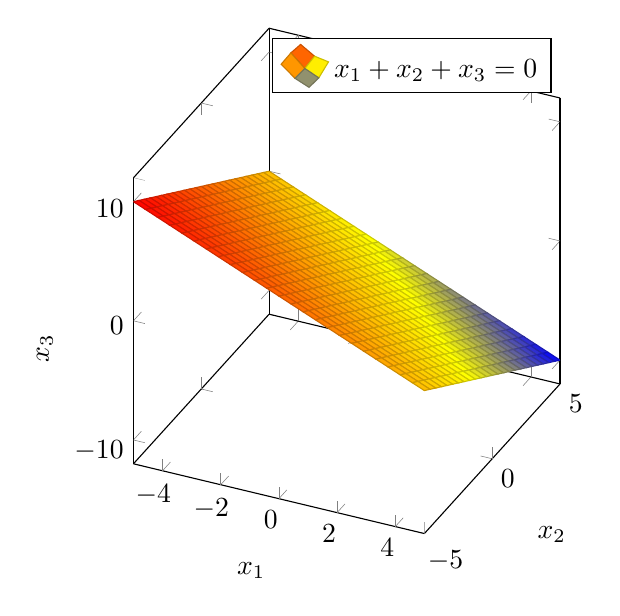
\begin{tikzpicture}
    \begin{axis}[
    width=7cm,height=8cm,
        xlabel = $x_1$,
    ylabel = {$x_2$},
    zlabel = $x_3$]
    \addplot3[
        surf,
    ]
    {-(x+y)};
    \addlegendentry{$x_1 + x_2 + x_3 = 0$}
    \end{axis}
    \end{tikzpicture}
	
	    \noindent\rule{\textwidth}{1pt}
	    
	\item \points{2} Given some $x_0 \in \R^n$, find the \emph{squared distance} to the hyperplane defined by $w^T x + b=0$.
	In other words, solve the following optimization problem:
	\begin{align*}
	\min_x& \|x_0 - x \|^2\\
	\text{s.t. }&w^Tx +b = 0
	\end{align*}
	(Hint: if $\widetilde{x}_0$ is the minimizer of the above problem, note that $\| x_0 - \widetilde{x}_0 \| = | \frac{w^T(x_0 - \widetilde{x}_0)}{\|w\|} |$. What is $w^T \widetilde{x}_0$?)\\
\\
    \noindent\rule{\textwidth}{1pt}
    {\bf Solution:}\\
    Let $x^*$ be the minimizer of the optimization problem, that is, let $x^*$ be the projection of $x_0$ onto the hyperplane. Then, the distance from $x_0$ to the hyperplane would be given (as the hint states) by the difference of the lengths of the projections of $x_0$ and $x^*$ onto the normal vector $w$:
    $$
    \|x_0 - x^*\| = \left| \frac{w^Tx_0}{\|w\|} - \frac{w^Tx^*}{\|w\|}\right| = \left|\frac{w^T(x_0 - x^*)}{\|w\|} \right|
    $$
    Since $x^*$ lies in the hyperplane, we have $w^Tx^* + b = 0$. Thus:
    $$
    \boxed{
    \|x_0 - x^*\|^2 = \left|\frac{w^Tx_0 + b}{\|w\|} \right|^2
    }
    $$
    \noindent\rule{\textwidth}{1pt}
    
\end{enumerate} 

A.10 For possibly non-symmetric $\mat{A}, \mat{B} \in \R^{n \times n}$ and $c \in \R$, let $f(x, y) = x^T \mat{A} x + y^T \mat{B} x + c$. Define $\nabla_z f(x,y) = \begin{bmatrix} \frac{\partial f(x,y)}{\partial z_1} & \frac{\partial f(x,y)}{\partial z_2} & \dots & \frac{\partial f(x,y)}{\partial z_n} \end{bmatrix}^T$.  
\begin{enumerate}
	\item \points{2} Explicitly write out the function $f(x, y)$ in terms of the components $A_{i,j}$ and $B_{i,j}$ using appropriate summations over the indices.
	\\
\\
    \noindent\rule{\textwidth}{1pt}
    {\bf Solution:}\\

    \noindent\rule{\textwidth}{1pt}
	\item \points{2} What is $\nabla_x f(x,y)$ in terms of the summations over indices \emph{and} vector notation?\\
\\
    \noindent\rule{\textwidth}{1pt}
    {\bf Solution:}\\

    \noindent\rule{\textwidth}{1pt}
	\item \points{2} What is $\nabla_y f(x,y)$ in terms of the summations over indices \emph{and} vector notation?
	\\
\\
    \noindent\rule{\textwidth}{1pt}
    {\bf Solution:}\\

    \noindent\rule{\textwidth}{1pt}
\end{enumerate}

B.2 \points{1} The \textit{trace} of a matrix is the sum of the diagonal entries; $Tr(A) = \sum_i A_{ii}$. If $A\in\mathbb{R}^{n\times m}$ and $B\in\mathbb{R}^{m\times n}$, show that $Tr(AB) = Tr(BA)$.\\

B.3 \points{1} Let $v_1,\dots,v_n$ be a set of non-zero vectors in $\mathbb{R}^d$. Let $V = [v_1,\dots,v_n]$ be the vectors concatenated. 
    \begin{enumerate}
        \item What is the minimum and maximum rank of $\sum_{i=1}^n v_i v_i^T$?
        \item What is the minimum and maximum rank of $V$?
        \item Let $A \in \mathbb{R}^{D \times d}$ for $D > d$. What is the minimum and maximum rank of $\sum_{i=1}^n (A v_i) (A v_i)^T$?
        \item What is the minimum and maximum rank of $AV$? What if $V$ is rank $d$?
    \end{enumerate}

\subsection*{Programming}

A.11 For the $A, b, c$ as defined in Problem 8, use
  NumPy to compute (take a screen shot of your answer):
  \begin{enumerate}
  \item \points{2} What is $A^{-1}$?
  \item \points{1} What is $A^{-1}b$? What is $Ac$?
  \end{enumerate}  


A.12 \points{4} Two random variables $X$ and $Y$ have equal
  distributions if their CDFs, $F_X$ and $F_Y$, respectively, are
  equal, i.e. for all $x$, $ |F_X(x) - F_Y(x)| = 0$. 
The central limit theorem says that the sum of $k$ independent,
zero-mean, variance-$1/k$ random variables converges to a (standard) Normal distribution as $k$ goes off to infinity.  
We will study this phenomenon empirically (you will use the Python packages Numpy and Matplotlib). 
Define $Y^{(k)} = \frac{1}{\sqrt{k}} \sum_{i=1}^k B_i$ where each $B_i$ is equal to $-1$ and $1$ with equal probability.
From your solution to problem 5, we know that $\frac{1}{\sqrt{k}} B_i$ is zero-mean and has variance $1/k$.
\begin{enumerate}
\item For $i=1,\dots,n$ let $Z_i \sim \mathcal{N}(0,1)$. If
  $F(x)$ is the true CDF from which each $Z_i$ is drawn (i.e.,
  Gaussian) and $\widehat{F}_n(x) = \frac{1}{n} \sum_{i=1}^n
  \1\{ Z_i \leq x)$, use the answer to problem 1.5  above to choose
  $n$ large enough such that, for all $x \in \R$, $ \sqrt{\E[
    (\widehat{F}_n(x)-F(x))^2 ]} \leq 0.0025$, and plot
  $\widehat{F}_n(x)$ from $-3$ to $3$. \\(Hint: use
  \texttt{Z=numpy.random.randn(n)} to generate the random
  variables, and \texttt{import matplotlib.pyplot as plt};\\
  \texttt{plt.step(sorted(Z), np.arange(1,n+1)/float(n))} to
  plot). 
\item For each $k \in \{1, 8, 64, 512\}$ generate $n$
  independent copies $Y^{(k)}$ and plot their empirical CDF on
  the same plot as part a.\\ (Hint: 
  $\texttt{np.sum(np.sign(np.random.randn(n,
    k))*np.sqrt(1./k), axis=1)}$ generates $n$ of the
  $Y^{(k)}$ random variables.) 
\end{enumerate}
Be sure to always label your axes. 
Your plot should look something like the following (Tip: checkout \texttt{seaborn} for instantly better looking plots.)

\begin{center}
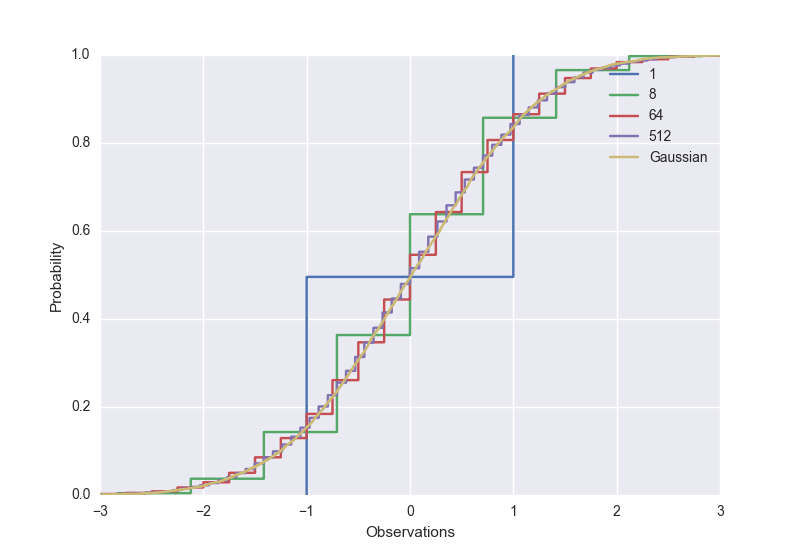
\includegraphics[width=4in]{full.png}
\end{center} 




\end{document}
